\documentclass{article}
\usepackage{graphicx}
\usepackage{amsmath}
\usepackage{enumerate}
\usepackage{chngpage}
\usepackage{amsmath}
\usepackage{graphics}
\usepackage{eurosym}
\usepackage{vmargin}
\usepackage{epsfig}
\usepackage{framed}
\usepackage{subfigure}

\pagenumbering{gobble}

\setmarginsrb{20mm}{0mm}{20mm}{25mm}{12mm}{11mm}{0mm}{11mm}
\begin{document}
{
	\large
\begin{center}
       
\includegraphics[scale=0.55]{shieldtransparent2}
\end{center}

\begin{center}
\vspace{1cm}
\large \bf {FACULTY OF SCIENCE AND ENGINEERING} \\[0.5cm]
\normalsize DEPARTMENT OF MATHEMATICS AND STATISTICS \\[1.25cm]
\large \bf {MID TERM EXAMINATION PAPER 2 2016} \\[1.5cm]
\end{center}

\begin{tabular}{ll}
MODULE CODE: MA4128 & SEMESTER: Spring 2016 \\[1cm]
MODULE TITLE: Advanced Data Modelling & DURATION OF EXAM: 1 hours \\[1cm]
LECTURER: Kevin O'Brien & GRADING SCHEME: 50 marks \\
&  \normalsize {20\% of total module marks} \\[0.7cm]

% EXTERNAL EXAMINER: Prof. Brendan Murphy &  \\[0.8cm]
\end{tabular}
\begin{center}
{\bf INSTRUCTIONS TO CANDIDATES}
\end{center}

{\noindent \\ Attempt All Questions
\\ Scientific calculators approved by the University of Limerick can be used. 
}
}

\newpage


%================================%

\section*{Question 1: Misscellaneouis}

\begin{enumerate}[(i)]
		\item In the context of statistical modelling, describe what is meant by Overfitting. You can support your answer with sketches.
		\item In the context of statistical modelling, describe what is meant by the Law of Parsimony
		%	\item[3.a] What is Multicollinearity? Describe the implications of Multicollinearity?
		%	\item[3.b] Contrast the uses of Training Data, Validation Data and Testing Data.
		\item In the context of statistical modelling, describe what is meant by overfitting?
		\item (2 Mars) What is Dimensionality Reduction
		\item (2 Marks) Compare and contrast dimensionality reduction techniques such as Variable Selection (e.g. Forward Selection and Backward Selection) with techniques such as Principal Componnent Analysis.
	\item(1 Mark) Suppose the odds of an outcome are 9. What is the probability of that outcome?
	\item (1 Makr) Suppose the probability of an outcome is 80\%. What is the odds of that outcome occuring?
	
	\item (2 Marks) Suppose that, out of a samle of 100 women and 100 men, 80 men drank alcohol in the last week, while 20 women drank alcohol in past week. Compute the odds ratio for Women to men
	
	\item Law of Parsimony
	\item 
	Ordinal and Multinomial Logistic Regression
	\item 
	Multicollinearity 
	\item 
	Tolerance and VIF

\end{enumerate}
\newpage
\section*{Question 2: Logistic Regression}


\begin{enumerate}[(i)]

\item (2 Marks) What is logistic regression? How does it differ from linear regression? Under what circumstances would you use it?

\item (2 Marks) Compare and contrast Binary Logistic Regression with Multinomial and Ordinal Logistic Regression.
	
\item (2 Marks) What is a dummy variable? Explain how it is used in Logistic Regression. Support your answer with an example.

\item What is a logit? how is it computed into a probability?

\begin{figure}[h!]
\centering
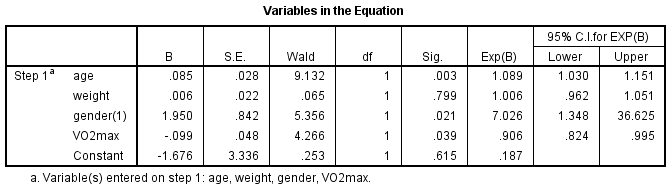
\includegraphics[width=0.9\linewidth]{waldtest}
\caption{}
\label{fig:waldtest}
\end{figure}



\end{enumerate}



	\[ \pi_i  =  \frac{e^{\eta_i}}{1 + e^{\eta_i}} \]
%================================%
\newpage
\section*{Question 3: Model Metrics and Variable Selection}

\begin{enumerate}[(i)]
	\item Given that there are $N$ predictor variables that can be used to predict an outcome. Consider a statistical model as a subset of these predictor variable. How many distinct models can be constructed (including a constant-term only model)
	\item AIC

\item Describe how you would use the Variance Inflation Factor to make an assessment about multicollinearity.
\item Describe how to use to the Akaike Information Criterion for model selection.

%	\item[3.g] Describe the process of model validation, with reference to training, validation and testing phases.
\item State two ways of methodically diagnosing the severity of multi-collinearity. How are these techniques related? How are they used to make decisions about the data?
\item Discuss a multiple regression technique could be affected by severe multicollinearity?

\item Explain what variable selection procedures are used for.
\item Compare and contrast three types of variable selection procedure.



\end{enumerate}


%================================%
\newpage
\section*{Question 4: Truncated, Censored and Missing Data}

\begin{enumerate}[(i)]
	\item (2 Marks) What is meant by missing data? Discuss the implications of Missing data in the context of a statistical analysis.
	\item (4 Marks) Missing Data is commonly classed into three different categories. What are these three categories? Compare and Contrast each of these three categories.
	
	\item (2 Marks) Consider the question in the figure below. This questionnaire is to be answered by parents of small children. 
	
\begin{figure}[h!]
\centering
\includegraphics[width=0.9\linewidth]{GUI}
\caption{}
\label{fig:GUI}
\end{figure}
	\item Compare and contrast the following types of missing data: Missing At Random, Missing
	Not At Random, Missing Completely at Random.
	
	\item What is meant by missing data? Discuss the implications of Missing data in the context of a statistical analysis.
	\item Compare and contrast Censored Data and Truncated Data
	\item Compare and contrast Missing Data, Interval Data and Censored Data.
	\item Describe two cases of censored data. Give a Practical exam for both cases.
\end{enumerate}


%================================%

\newpage
\section*{Question 5: Principal Component Analysis}


\begin{enumerate}[(i)]
	\item 
	What is PCA. 
	\item Methods of choosing number of components to extract.
	
	\item KMO
	Bartlett

	
	\item What is the KMO statistic? Describe how to interpret the KMO statistic.
	\item What is the Bartlett Test of Sphericity used for?
	\item varimax, quartimax and equamax are the commonly used methods in a certain procedure. What is this procedure? What is the purpose of the procedure.
	Which method is the most commonly used?
	\item Describe how to use a Scree plot in the context of dimensionality reduction techniques.
	
	
%	\item The KMO is used to measure what characteristic of the data. Explain how the KMO
%	measure should be interpreted.
	\item Briefly describe the Bartlett Test for Sphericity, with reference to the null and alternative
	hypotheses, and how those statements relate to the purpose of the test.
	\item (3 $\times$ 2 Marks) Discuss three techniques for determining the appropriate number of principal components.
	
	
	\item What is the purpose of a principal component analysis? Compare and contract PCA and variable selection procedures such as backward selection. 
	
\end{enumerate}\begin{figure}
\centering
\includegraphics[width=0.7\linewidth]{unrotated}
\caption{}
\label{fig:unrotated}
\end{figure}

%================================%
\begin{figure}
\centering
\includegraphics[width=0.7\linewidth]{rotated}
\caption{}
\label{fig:rotated}
\end{figure}


\end{document} 